\section{Introduction}\label{intro}
In Astronomy, instruments with higher angular resolution allows us to measure ever smaller structures in the sky. For Radio frequencies, the angular resolution is bound to the antenna dish diameter, which puts practical and financial limitations on the highest possible angular resolution. Radio Interferometers get around this limitation by using several smaller antennas instead. Together, they act as a single large antenna with higher angular resolution at lower financial costs compared to single dish instruments.

Retrieving the observed image for Radio Interferometer becomes difficult. The Interferometer does not measure pixels of the sky. Instead, it measures an incomplete set of Fourier components. Each antenna pair samples a point in the Fourier Domain. To retrieve the image, a reconstruction algorithm has to find the Fourier Transform of the measurements, even though it is missing information. This forms an ill-posed inverse problem. There are potentially many images that fit the measurements of a Radio Interferometer. From the measurements alone, we do not know which of the possible images was actually observed.

Image reconstruction algorithm which tackle the ill-posed inverse problem. We have two dimensions, reconstructing an image which is as close as possible to the truly observed one, and finding an image as fast as possible.

New Radio Interferometers.

Image reconstruction algorithms therefore have to find the most likely image of a measurements.

Finding an image as fast as possible
Finding the most likely observed image.

What this project does


\subsection{Radio Interferometric Inverse Problem}
What is a baseline.
What is an Observation. Over a time window. Create an image over several hours of measurements.
Channels, Polarization.

The inverse problem

Inverse Problem, We have measurements and want to find the image matching the measurements. Incomplete, there are potentially infinite number of images fitting the measurements. This forms an Ill-Posed inverse problem. 

Solving this ill posed inverse problem with image reconstruction


Radio Interferometers measure Fourier Components of the Sky. We have a Fourier relationship between measurements and image.

Image reconstruction problem shown in figure \ref{intro:inversefig}
Measurements in the Fourier Domain in figure \ref{intro:inversefig:uvspace}. Each dot represents a measurement of the Radio Interferometer. Incomplete, we do have holes in the UV space. But also a very large number of measurements. Non-uniform sampling pattern in the Fourier space. The sampling pattern is defined by the instrument, we have pockets with high number of samples, and areas with few samples. We have "Holes" in the Fourier space, meaning we do not have all the information available for the Nyquist-Shannon sampling rate. In essence, we are missing information for the image.

Reconstructed image \ref{intro:inversefig:reconstruction}



\begin{figure}[htp]
	% preliminary
	\sbox\twosubbox{%
		\resizebox{\dimexpr.9\textwidth-1em}{!}{%
			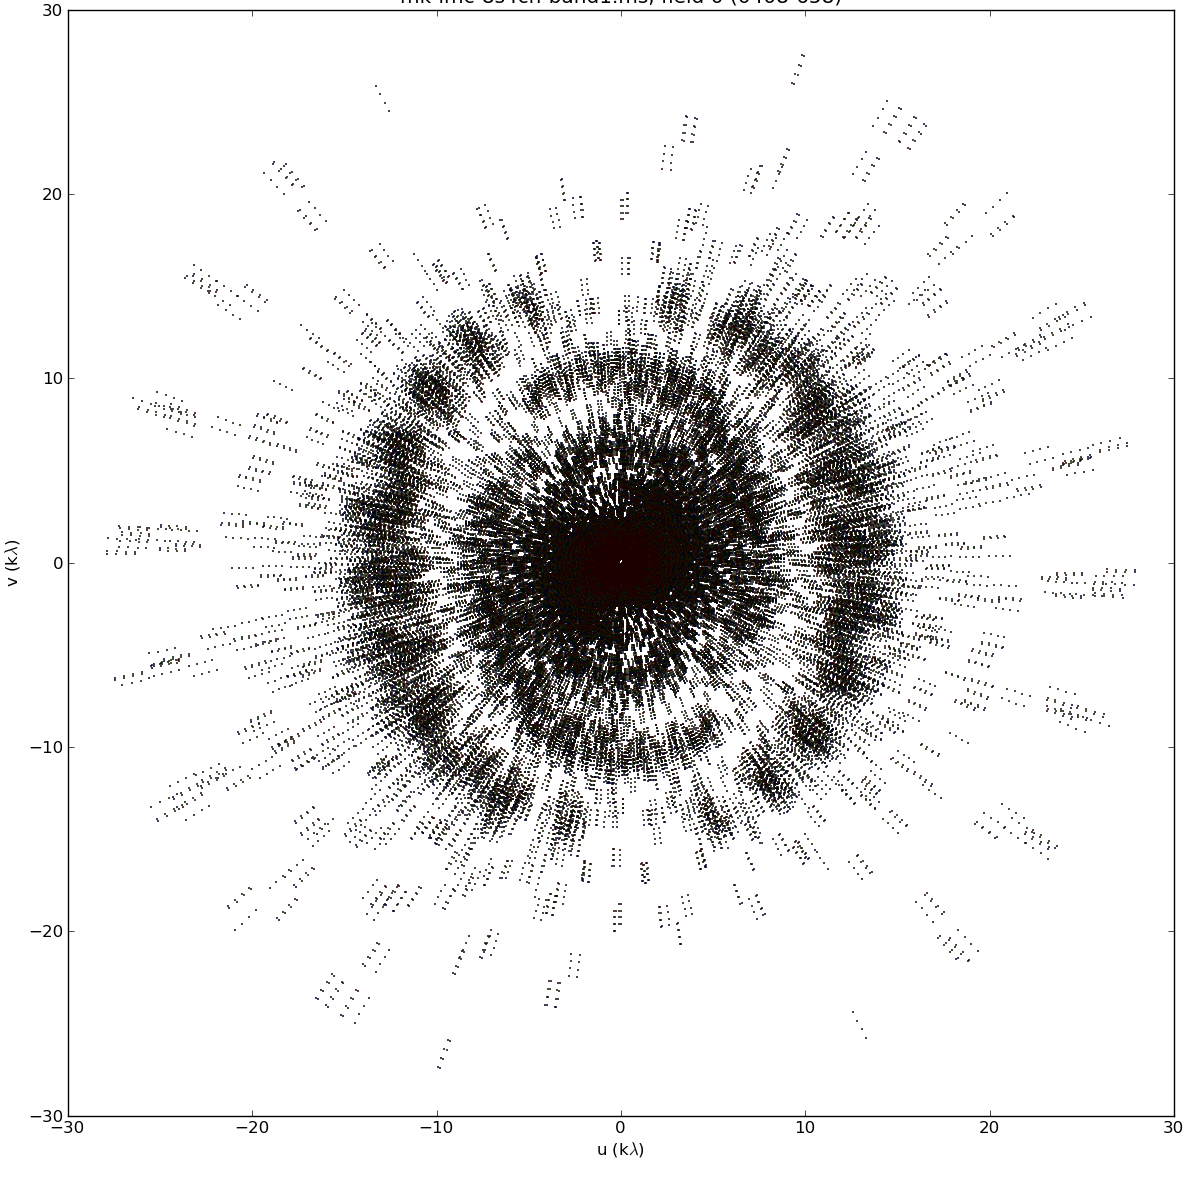
\includegraphics[height=3cm]{./chapters/01.intro/meerkat_uv2.png}%
			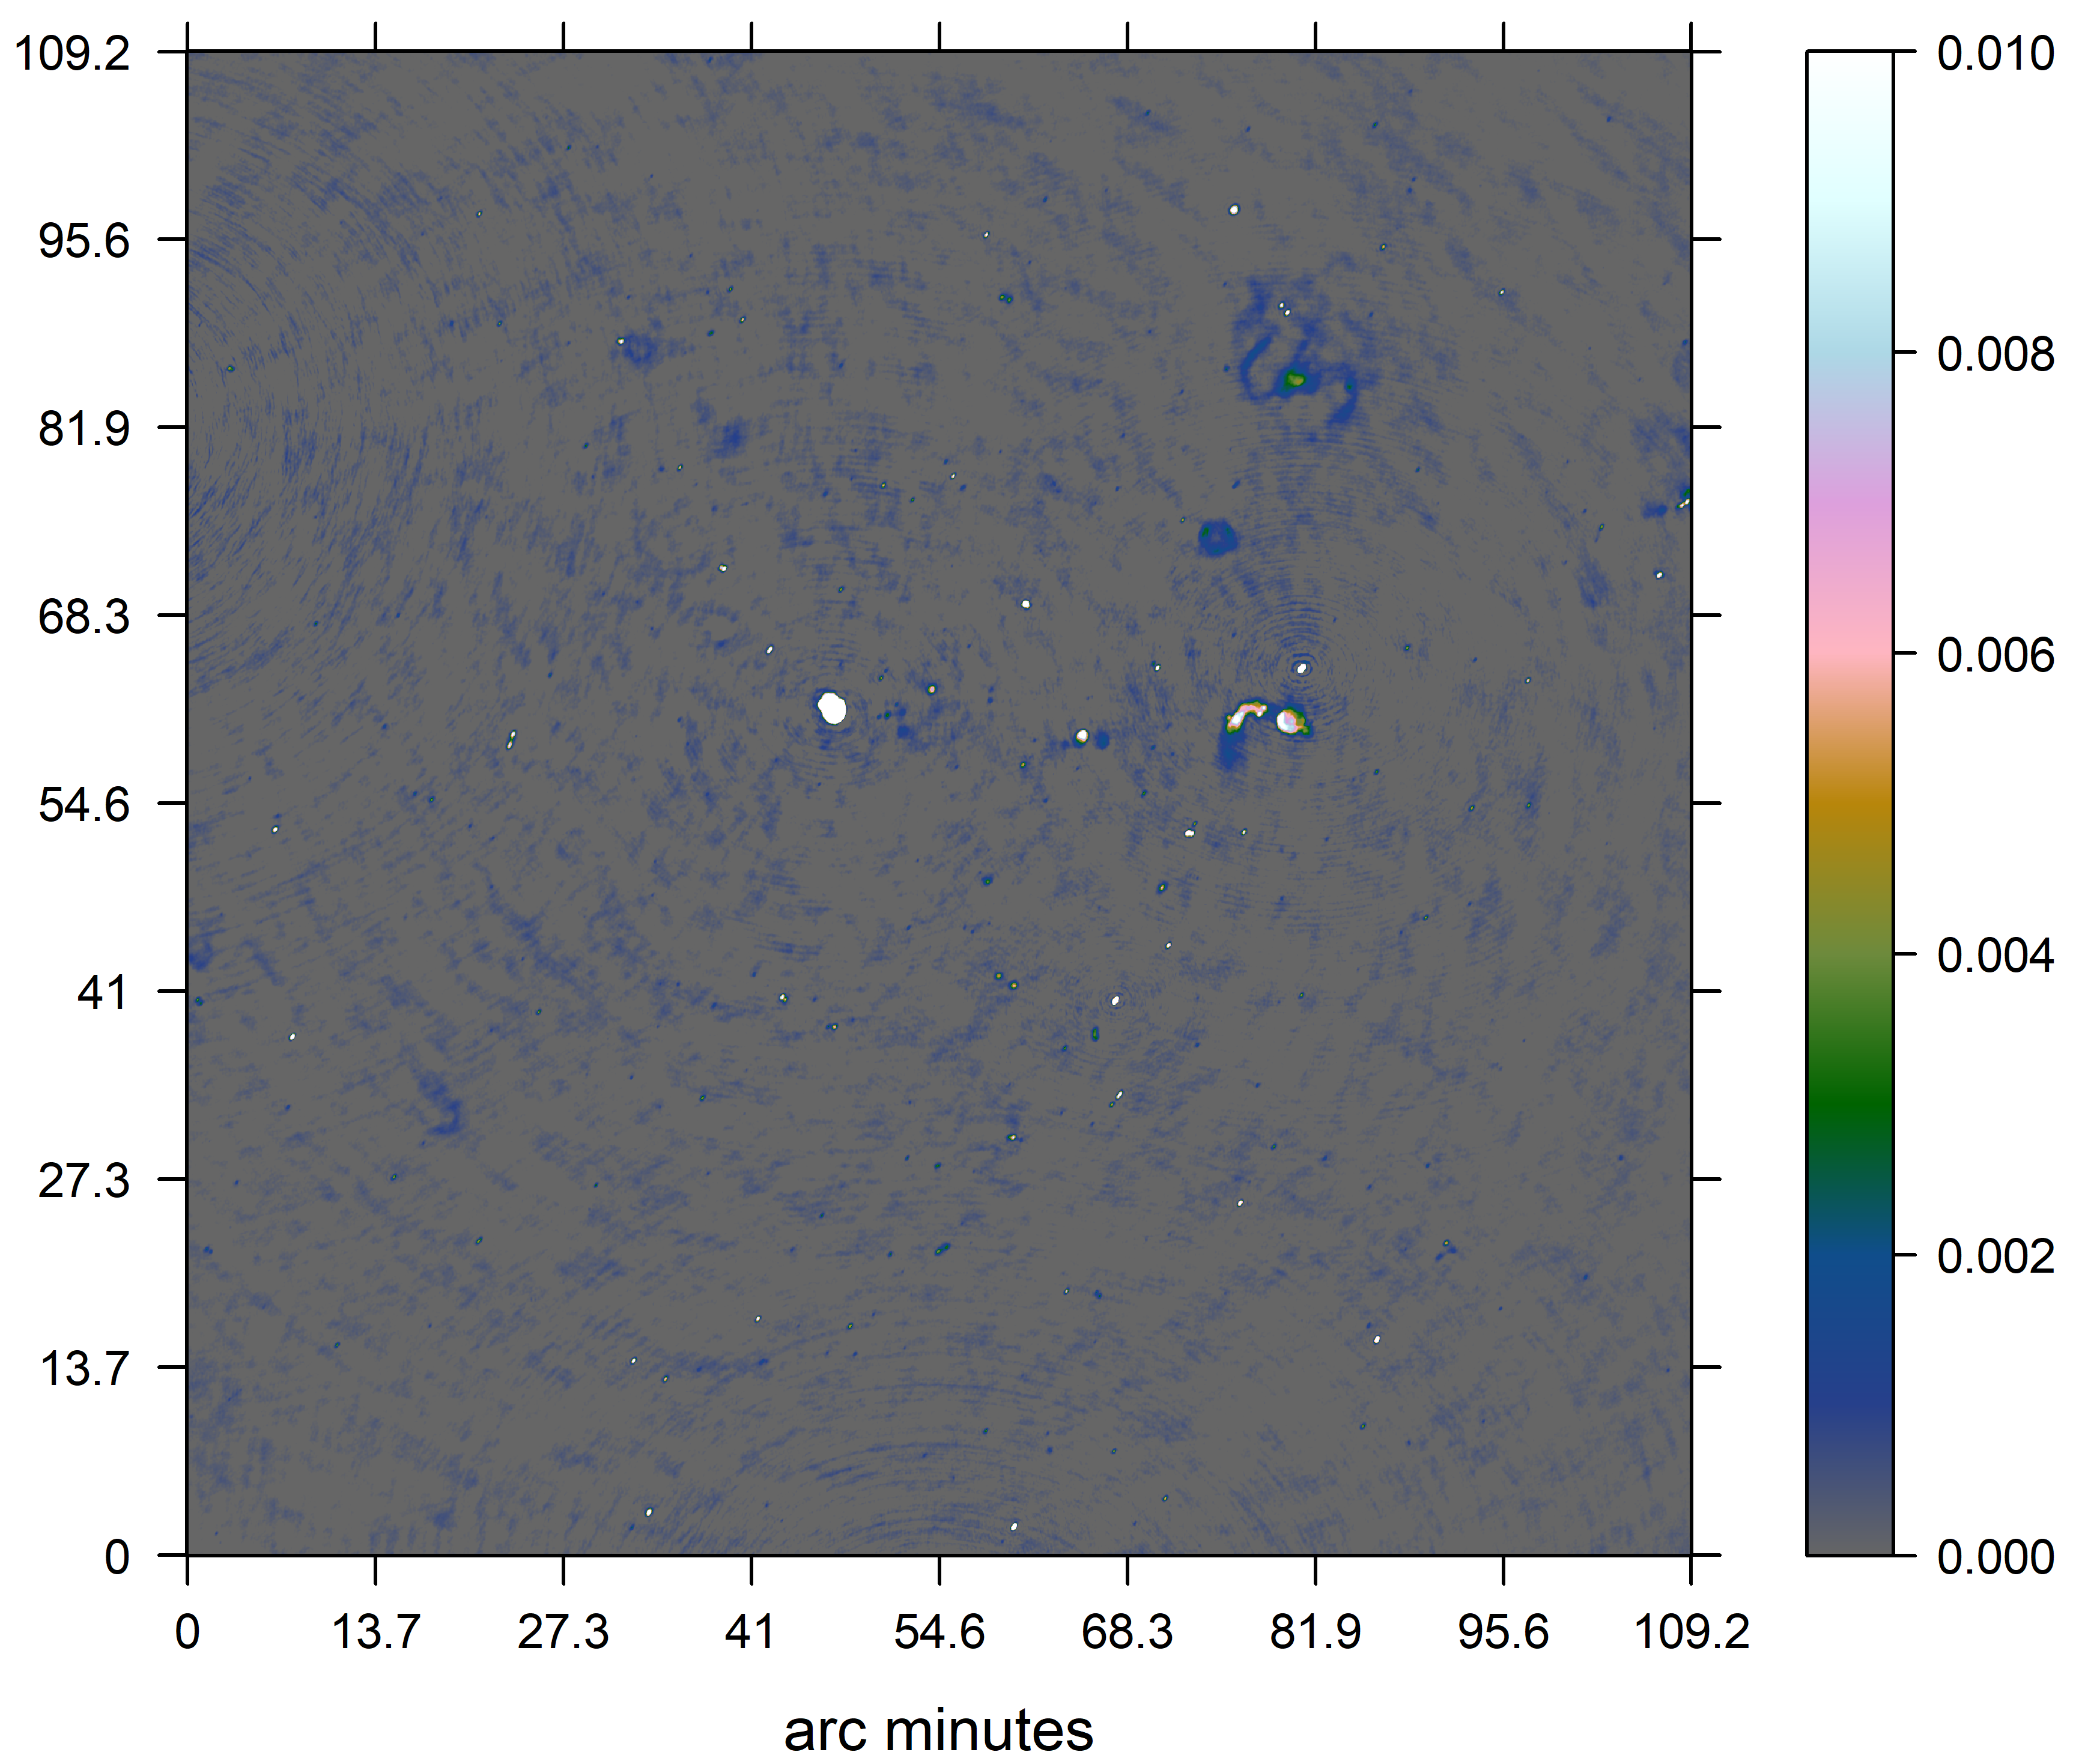
\includegraphics[height=3cm]{./chapters/01.intro/meerkat_clean2.png}%
		}%
	}
	\setlength{\twosubht}{\ht\twosubbox}
	
	% typeset
	\centering
	\subcaptionbox{Measurements of the MeerKAT Radio Interferometer.\label{intro:inversefig:uvspace}}{%
		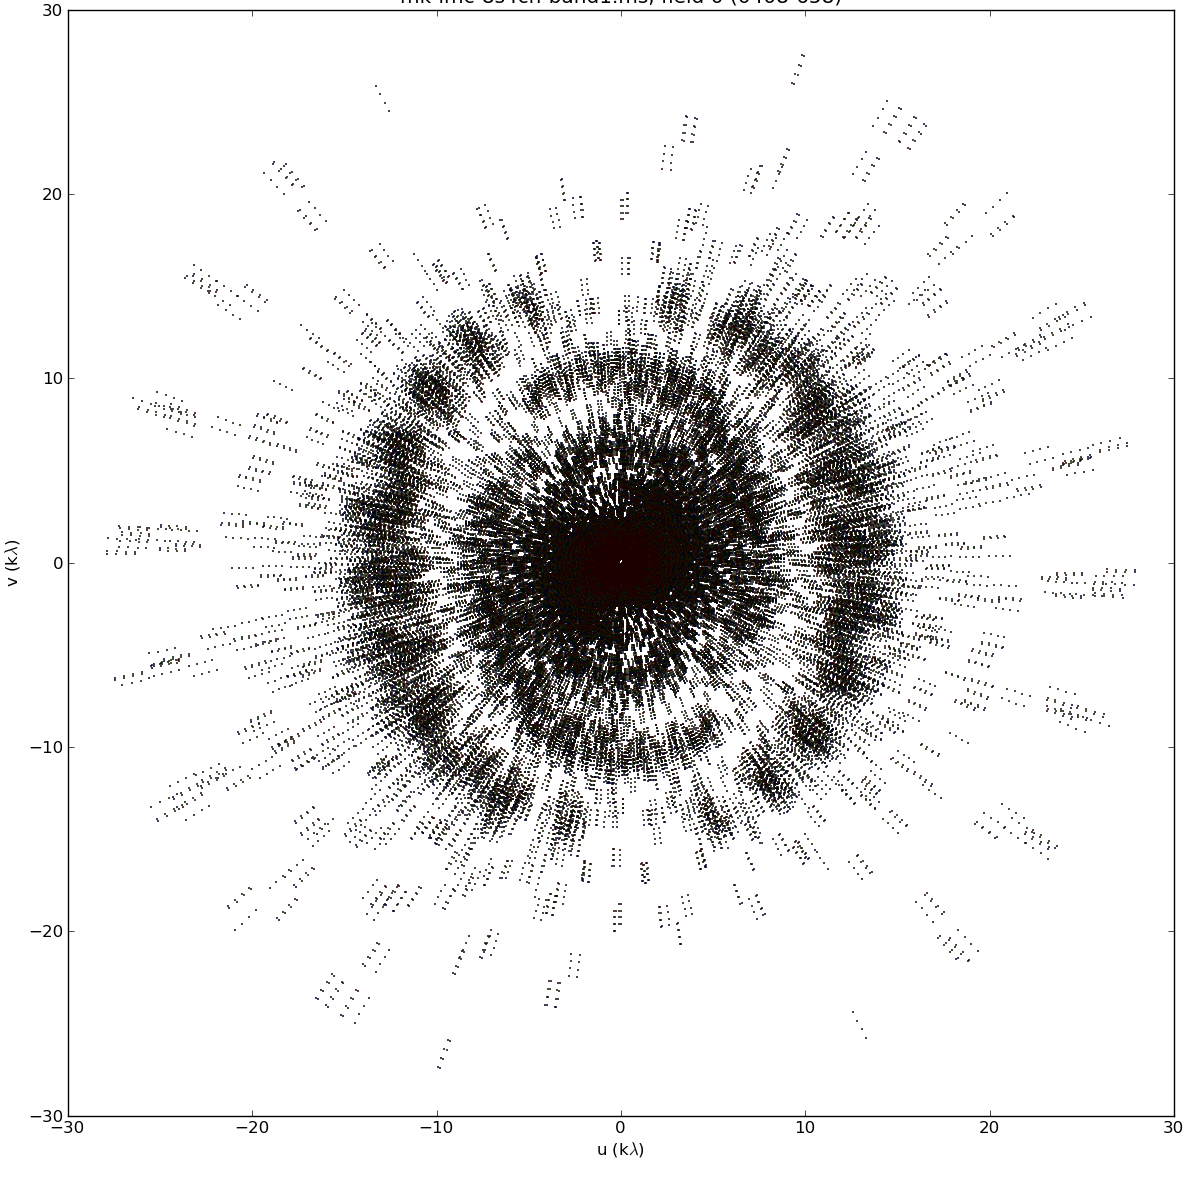
\includegraphics[height=\twosubht]{./chapters/01.intro/meerkat_uv2.png}%
	}\quad
	\subcaptionbox{A reconstruction which fits the observation.\label{intro:inversefig:reconstruction}}{%
		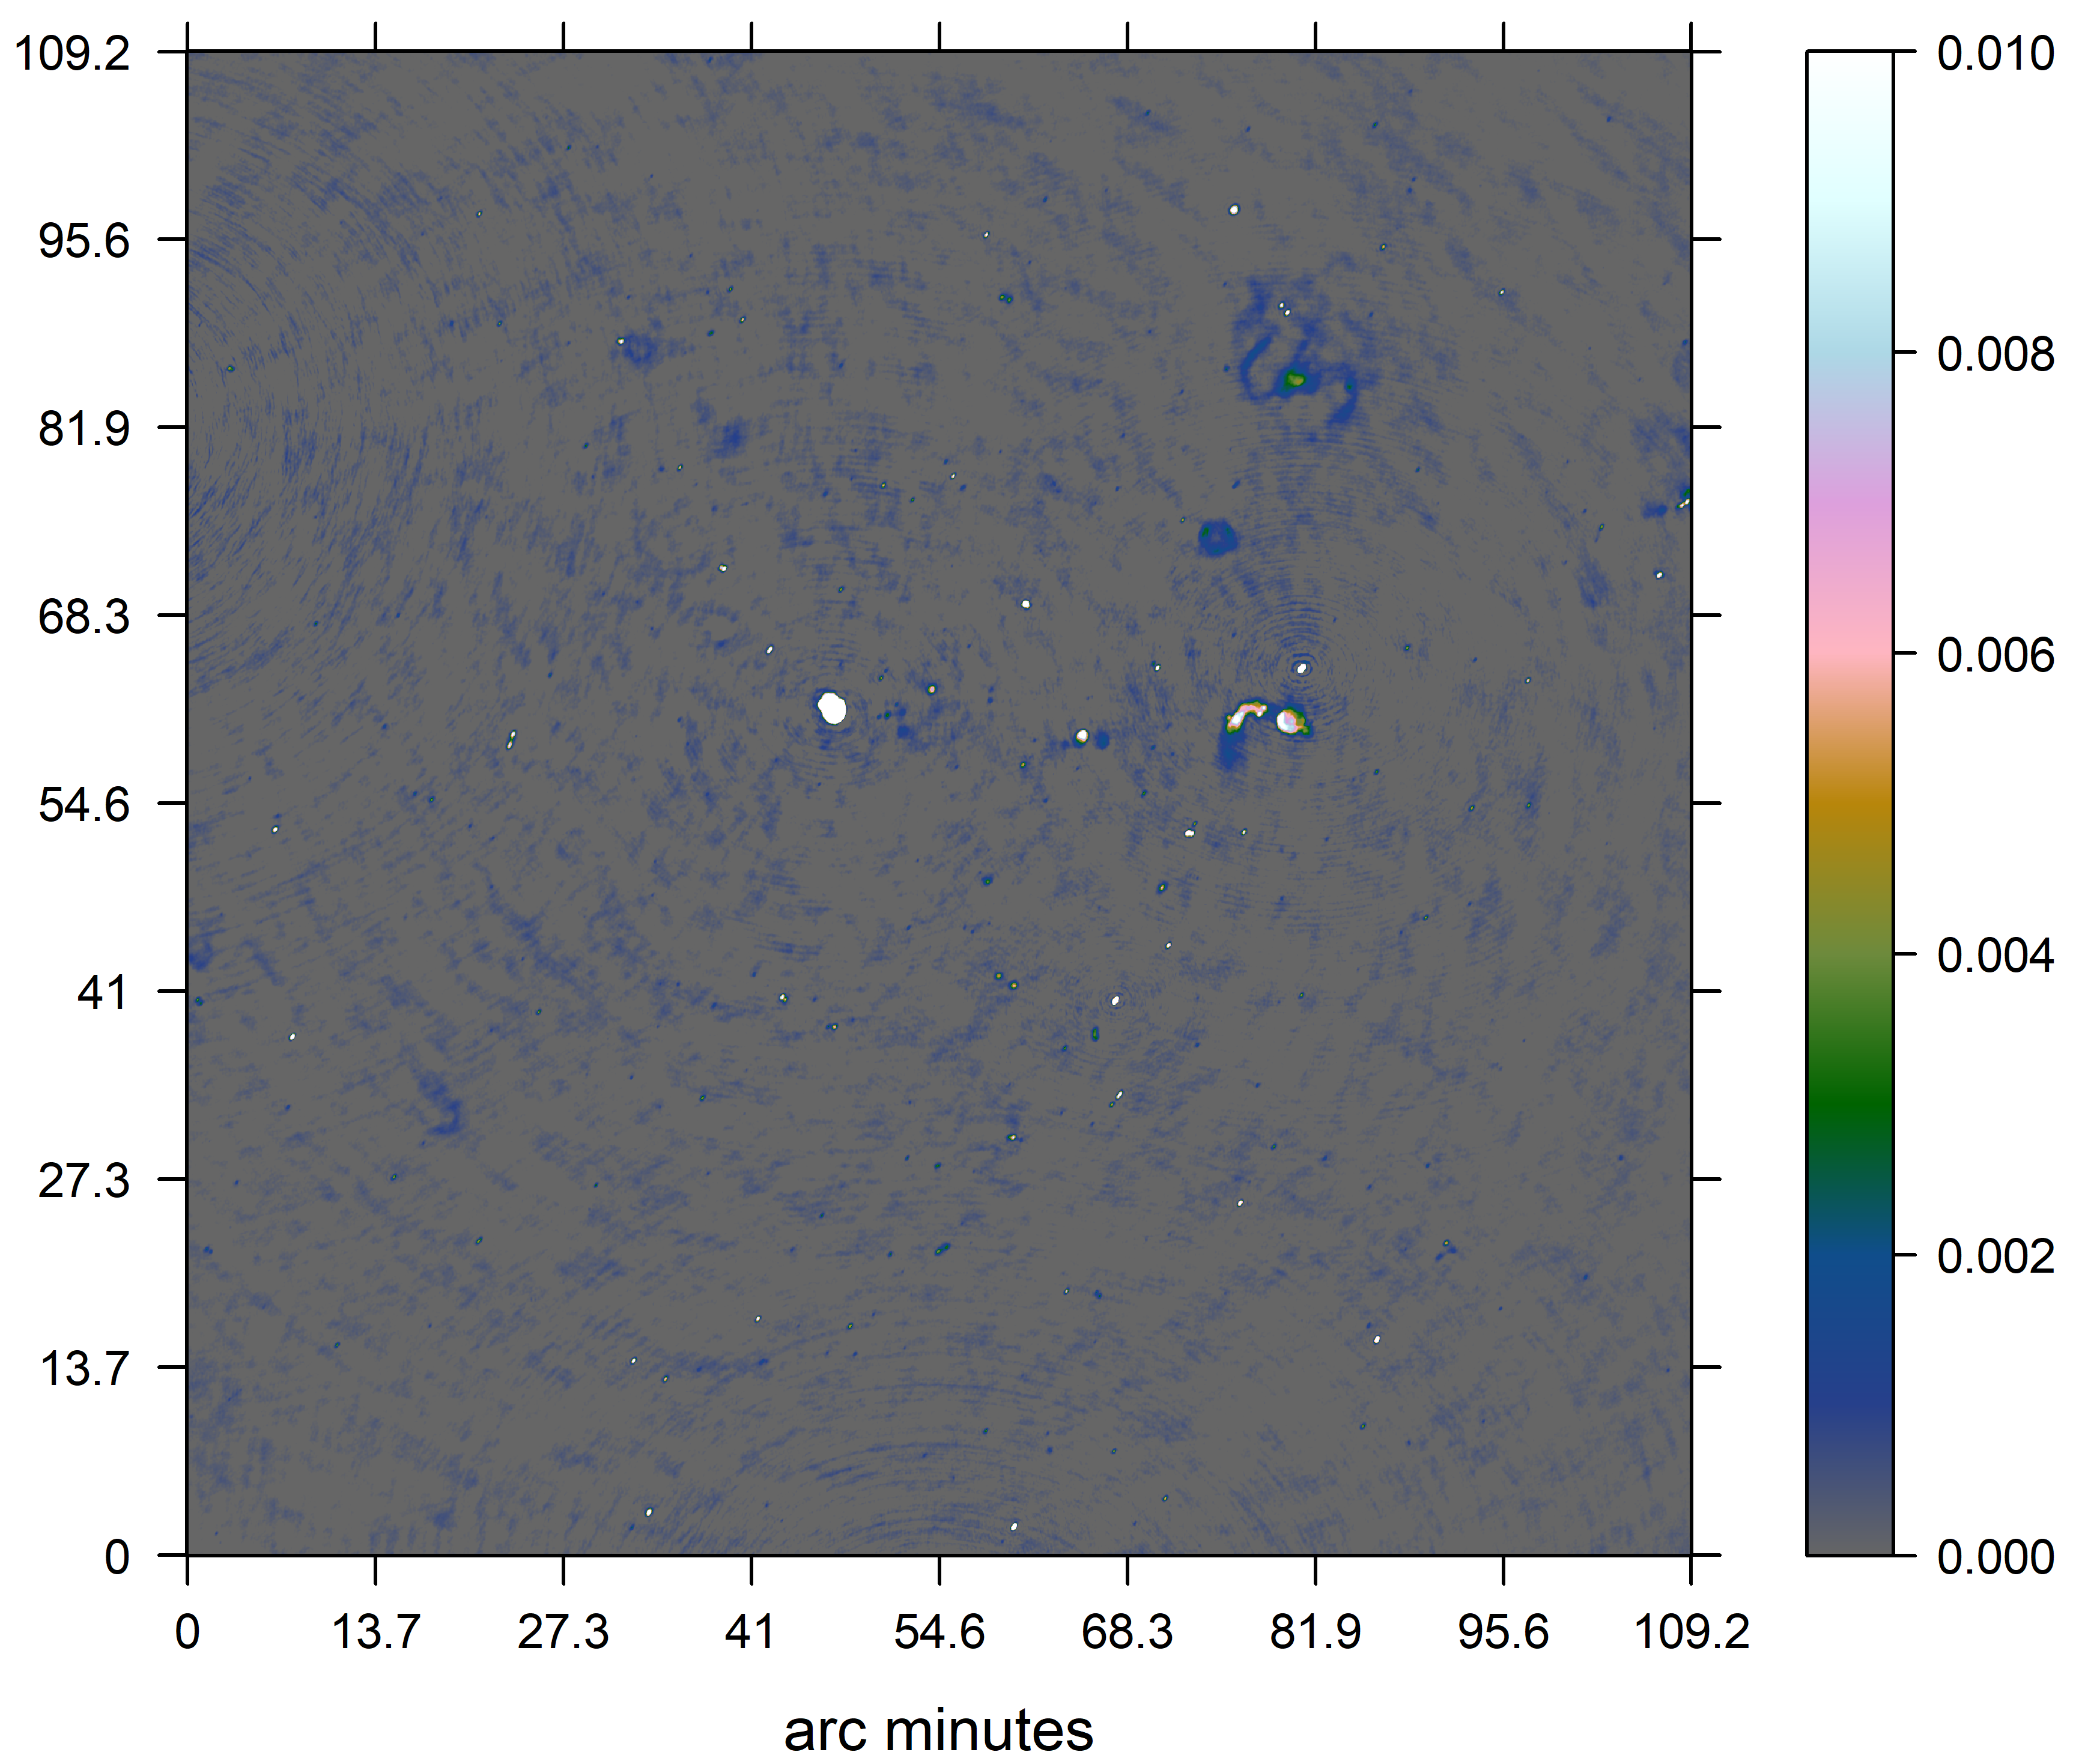
\includegraphics[height=\twosubht]{./chapters/01.intro/meerkat_clean2.png}%
	}
	\caption{The Image Reconstruction Problem}\label{intro:inversefig}
\end{figure}



Overdetermined problem, we have magnitudes more Visibilities than Pixels in the image. But noise and holes in the 


Or more formally in equation \eqref{intro:inverseproblem}


\begin{equation}\label{intro:inverseproblem}
V(u, v, w) = \int\int \frac{I(x, y)}{\sqrt{1 - x^2 - y ^2}} e^{2 \pi i [ux+vy+ w(\sqrt{1 - x^2 - y ^2} - 1)]} \: dx \: dy
\end{equation}

3d Fourier Relationship.

w-projection.
Our


\subsection{Radio Interferometric Image Reconstruction}

Solving the Ill-Posed inverse problem
Whole system.
From measurements to image reconstruction contains many different steps. In this project, we concern ourselves with the image reconstruction

\begin{figure}[h]
	\centering
	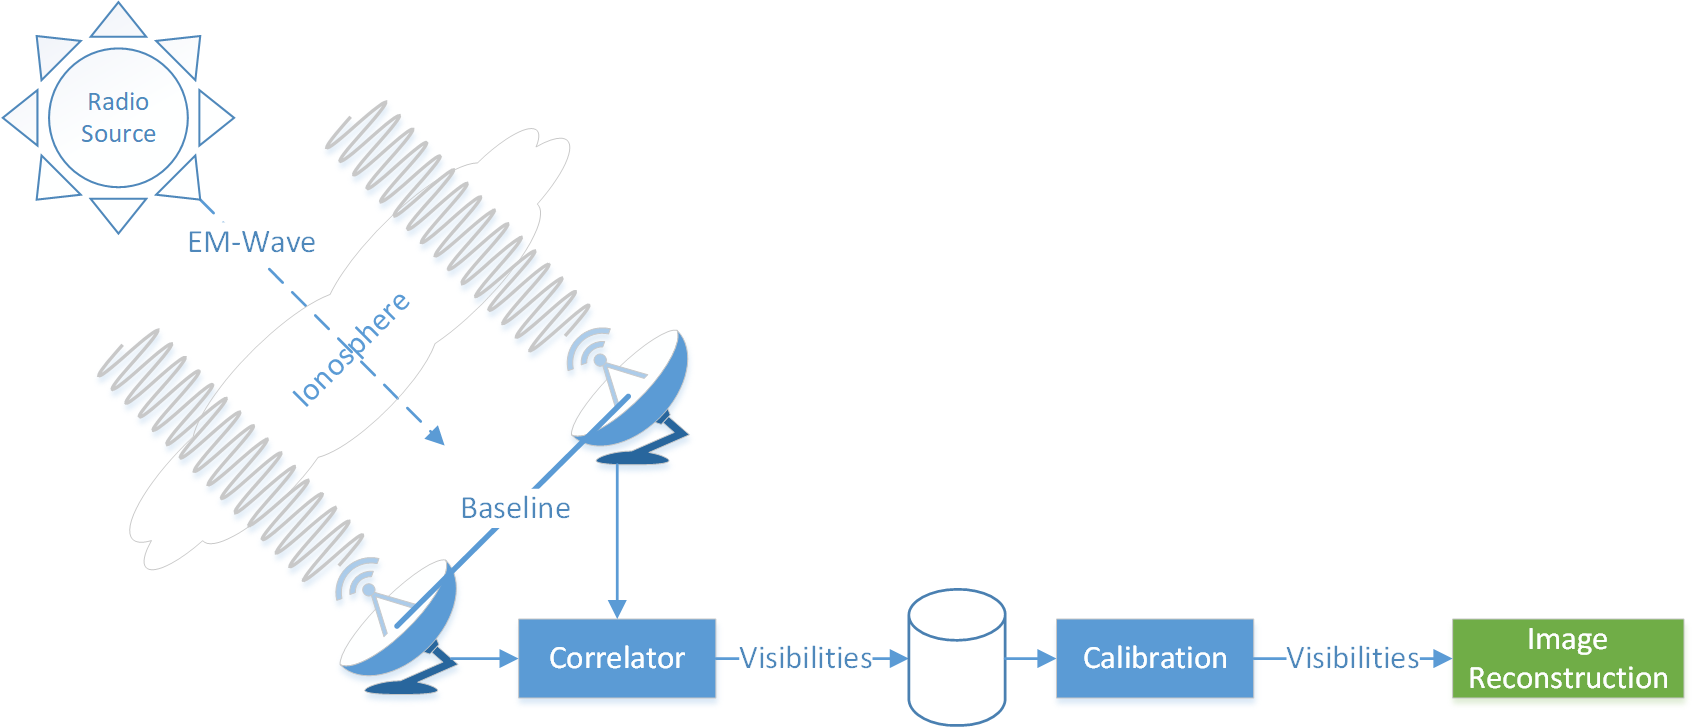
\includegraphics[width=0.80\linewidth]{./chapters/01.intro/system.png}
	\caption{Interferometer System}
	\label{intro:system}
\end{figure}

Calibration is not directly
Bad calibration can introduce a special error in the image.

Different ways of formulating the image reconstruction problem:
Interpolating the missing Visibilities
Deconvolution (also called "Minor Cycles")
Finding an image which fits the measurements

\subsubsection{The Major Cycle Architecture}
State of the art architecture used for reconstructing images. It Models the problem as deconvolution, and it needs three Operations:
\begin{itemize}
	\item Gridder
	\item FFT
	\item Deconvolution
\end{itemize}

The full algorithm is done 

\begin{figure}[h]
	\centering
	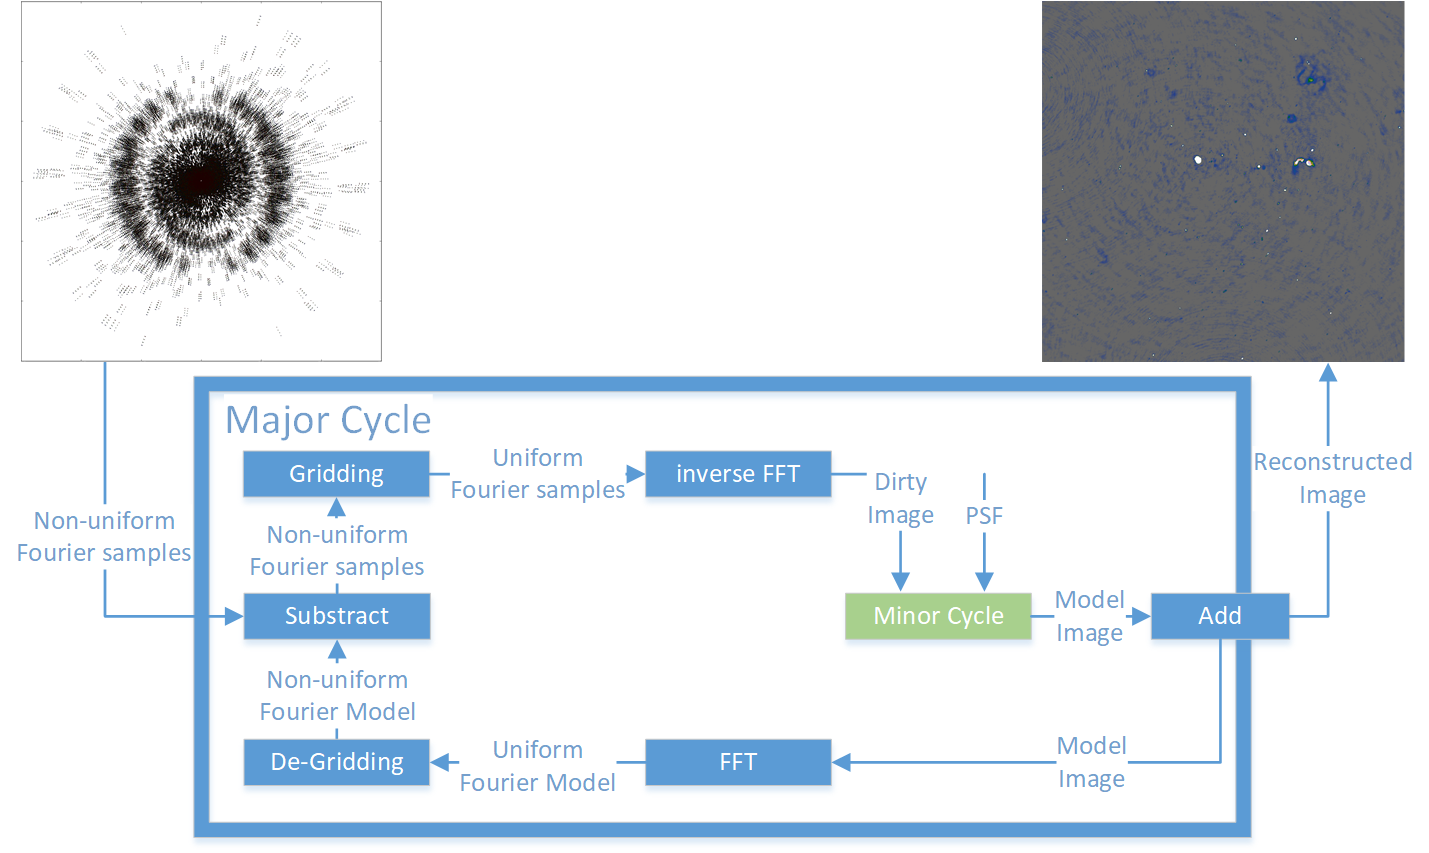
\includegraphics[width=0.80\linewidth]{./chapters/02.hypo/Major-Minor3.png}
	\caption{The Major Cycle Architecture}
	\label{intro:major}
\end{figure}

\subsubsection{ Deconvolution}
Other algorithms, mainly CLEAN
CLEAN




\subsection{Large scale Reconstruction Problem of MeerKAT}
New class of radio interferometers produce an ever increasing number of data.


Bottlenecks.
The Problem of Computation vs Quality
Image is magnitudes smaller than input data

Deconvolution with CLEAN.

Mostly Shared-Memory systems, large single machines.

GRIDDING Problem. The $w$-component of the Visibilities made this difficult. 

w-stacking, lately IDG. This has made the Gridding more efficient.

Use IDG to Distribute the Gridding.




CLEAN deconvolution still hard to parallelize.


\subsubsection{Gridding on the GPU}

\subsubsection{Theory of Compressed Sensing}











